\documentclass{vldb}
\usepackage{balance}
\usepackage{url}
\usepackage{algorithm2e}
\usepackage{color}
\usepackage{graphicx}
\usepackage{array}
\usepackage{adjustbox}
\usepackage{times}
\usepackage{booktabs}
\usepackage{multirow}
\usepackage{subfigure}
\usepackage{flushend}
\usepackage{float}

\usepackage{listings}
\lstset{language=Java,
basicstyle =\small,
xleftmargin=0.05\linewidth,
xrightmargin=0.05\linewidth}

\lstMakeShortInline[language=java]{|}

\newcommand{\ol}[1]{\texttt{\small #1}}
\newcommand{\OL}[1]{\texttt{\textbf{#1}}}


\newcommand{\inner}[2]{\left\langle #1,#2 \right\rangle}
\newcommand{\vect}[1]{\boldsymbol{#1}}
\newcommand{\xy}[0]{(\vec{x},y)}
\newcommand{\w}[0]{\vec{w}}
\newcommand{\argmin}[1]{\underset{#1}{\operatorname{argmin}}}

\newcommand{\note}[2]{[\textcolor{red}{\textbf{#1:} \emph{#2}}]}
\newcommand{\memo}[1]{[\textcolor{blue}{\textit{#1}}]}


\newcolumntype{R}[2]{%
    >{\adjustbox{angle=#1,lap=\width-(#2)}\bgroup}%
    l%
    <{\egroup}%
}
\newcommand*\rot{\multicolumn{1}{R{90}{1em}}}% no optional argument here, please!


\newcommand{\eat}[1]{}

\begin{document}


\title{LLAP: Live Long and Process}

\numberofauthors{1} 
\author{
\alignauthor
??$^m$, Gopal Vijayaraghavan$^h$, Gunther Hagleitner$^h$, Prasanth Jayachandran$^h$, \\ 
Sergey Shelukhin$^h$, Siddharth Seth $^h$
\\
{\large \emph{$^h$: Hortonworks, $^m$: Mentor Professor}}
}

\maketitle

\begin{abstract}
Apache Hive has turned SQL into a first-class citizen in the ecosystem surrounding Apache Hadoop.
The popularity of Apache Hive has been driven by the vast improvements in performance brought in
by the the addition of a new DAG based execution engine, vectorized operator pipelines, a cost based
optimizer and compressed columnar storage. Continuing the journey towards ever faster queries,
as the needle swings closer to sub-second scale, several historical tradeoffs have to be revaluated.  
In addition to pure performance goals, there are new opportunities offered by the evolution of compute, 
storage and networking hardware to be taken advantage of.


In this paper, we introduce LLAP, an \emph{in-memory SQL acceleration framework} for Apache Hive, designed
to run low-latency SQL workloads for ad-hoc querying, Business Intelligence analytics and periodic reporting.
Central to this design are long lived processes, which provide an in-memory SQL execution substrate which draws
data out of a completely automated caching layer. The long-lived nature of these LLAP instances, retains the runtime profile
information of several short queries to provide the JVM JIT long term context to optimize the execution engine
using \emph{SIMD} instructions to suit the exact users' data model \& workload.


Even though low-latency execution is the primary performance goal, it is the combination of failure tolerance, 
internal pre-emption model based on dynamic query fragment priority, user-transparent replicated data/index fragment
caching \& eviction, ability to maintain isolation for update/delete ACID transactions and perform out-of-core joins 
that makes \emph{LLAP} an entirely different beast from the other open source solutions which offer performance at the cost
of necessary functionality.


LLAP's design draws from the experiences learned from deployments of scale of Apache Hive \& Apache Tez. We complement
the qualitative accounts of LLAP's development with quantitative experimental evidence that the dragon of latency in
a multi-tenant environment can have its long tail cut.


\end{abstract}

\section{Introduction}

The enterprise data warehouse, once a workhorse of the data analytics companies is slowly merging with the once exotic technologies used for large scale data analytics, giving birth to innovations such as Hive, which has turned HiveQL into a de-facto SQL implementation dialect. This popularity has come on the heels of a reduction in cost and has ridden on the coat-tails of the \emph{schema-on-read} model primarily brought by NoSQL data sources. The familiarity of SQL and the flexibility of storage brings us to the present day, where SQL-on-Hadoop is on its rise as the preferred data access model garnering adoption from companies which use either SQL or Hadoop heavily.

In this paper, we inspect this vibrant ecosystem through the lens of Apache Hive, as this provides the perspective for introducing LLAP. Refer Section~\ref{sec:relwork} for a broader comparison of the related or competing projects, which were undeniably also inspired by the success of Hive and have provided goalposts to aim for or pitfalls to avoid in our quest to improve Apache Hive. 

Hive was initially a SQL-like layer designed over MapReduce, but has since evolved into a mature engine with advanced OLAP capabilities required for a modern data analytics platform.
The undeniable success of Hive and its widespread adoption demanded innovations along the way, including adopting columnar storage \cite{ORC}, designing a fully fault-tolerant DAG framework \cite{tez}, adopting an advanced cost based optimizer \cite{calcite} and adding ACID insert/update/delete transactions with strong consistency. This phase of the journey resulted in Hive establishing itself as the tool of choice of SQL ETL workloads, but also allows ad-hoc queries and reporting with greater efficiency and higher performance than the original MapReduce based batch model.

Hive also established itself as the single system of record for metadata for tabular data across the ecosystem, with nearly all SQL-on-Hadoop open source projects building bridge mechanisms to access Hive data as a first-class data source and in general, tailor their SQL dialects to match. Over the period of half a decade, the length of the average query kept shrinking from hours down to a few seconds, reducing more than 100x as part of the Stinger\cite{tez} initiative. This brings Hive's performance close to the ballpark for business intelligence workloads, which demand latencies better measured in milliseconds.

In this paper, we introduce LLAP, the innovation over the existing foundations of Hive, which cuts through layers of overheads which have kept Hive out of the sub-second category. The system combines all the advantages of Apache Hive and Tez with an in-memory acceleration layer which brings common low-latency workloads to acceptable speed, while adding better concurrency models for multi-tenancy. LLAP is not an execution engine by itself, but is an accelerator which relies on the emergence of large memory machines to speed up queries.

LLAP was built under some fundamental assumptions:
\begin{enumerate}
\item Low-latency is the first goal, but not the only one
\item Failure tolerance is critical 
\item Multi-query concurrency is critical 
\item Production clusters are always busy and need forced pre-emption
\item Temporal data access patterns are common
\item Data will overflow caches and working sets 
\item Caches have to be automatic, including eviction 
\item Elasticity is necessary - shed capacity during off-peak hours
\item Automatic service discovery brings elasticity 
\item Strong security models need user/framework process boundaries 
\item Hybrid execution is necessary for process boundaries
\end{enumerate}

LLAP is unique in its pursuit of the low-latency goals as it does not try to reinvent a completely new SQL engine. It offers an execution algebra layer which interacts with the Hive execution engine, with dynamic decisions on whether a query or even parts of a query render down into the LLAP query fragments. This brings it closer to production readiness than other solutions which offer an all-or-nothing framework, which takes away key features of Hive like strong security models or failure tolerance as part of the choice.

The query fragment independence offers some of the same advantages to any engine which can use LLAP as a data source. This raises the possibility that LLAP can serve as a pluggable data source for 
distributed task execution systems such as PIG \cite{pig}, Flink\cite{flink}, and Spark\cite{spark}, allowing for secure process separation for column or row-level security. Exporting LLAP as a data source with security built-in, allows for geographically distributed queries, with a data-model that spans multiple geo-locations and independent federated query execution.

Beyond discussing the execution mechanisms of LLAP, we demonstrate its abilities to accelerate queries, provide security separation and provide concurrency control for busy clusters advantages over other execution engines of Tez, we demonstrate its competence to support Hive, Pig, and Spark, by running standard benchmarks such as TPC-H and TPC-DS, and production workloads from Yahoo!. 

The rest of this paper is organized as follows: 
Section~\ref{sec:hist} provides some more historical context, and rationale for the design, 
while Section~\ref{sec:arch} introduces architectural underpinnings of LLAP. 
Section~\ref{sec:elasticity} discusses the deployment model of LLAP and the elasticity mechanisms of LLAP, 
Section~\ref{sec:cache} discusses the cache implementation of LLAP, 
Section~\ref{sec:orchestration} discusses the orchestration and task distribution implementation of LLAP including failure tolerance,
Section~\ref{sec:concurrency}discusses the internal resource management which brings better concurrency to LLAP,
Section\ref{sec:exp} is devoted to the experimental evalution and measurements from real-world deployments,
We conclude by discussing future and related work in Sections~\ref{sec:futwork} and \ref{sec:relwork}, 
and conclude in Section~\ref{sec:conclusions}

\section{Architecture}


\emph{LLAP}, as the name suggests is a long running collection of persistent daemons, which by virtue of being always on side-steps the
overheads of interacting with a large scale resource manager such as YARN\cite{YARN} while executing very short running queries. 

In addition to
that, the long running nature of the processing framework allows for the JDK Hotspot profiling optimizer to collect enough runtime information
to compile the core vectorized loops into \emph{SIMD} native code. To feed this CPU efficient operator pipeline, the data fetching from the storage layer
had to be revamped to buffer into temporary buffer pools so that the operator pipeline is never starved by the vagaries of the networked file
system layer. Since several processing queries share the same data sets, it is incredibly wasteful to discard buffer pools after execution which
naturally led into a cache model which can keep the uncompressed buffers in memory. To reduce the amount of data being fetched for caching, the 
buffers are held as independent columns so that the fetcher can populate a fraction of columns to match the column projections which were involved
during the scan.  The columnar buffers are not unpacked into rows during caching, so the cache maintains all the compression characteristics of the columns such 
as RLE, delta or dictionary encoding. To avoid large GC pauses associated with a large number of indepenent heap objects present in the process heap, 
these cache objects are maintained an off-heap allocator which can be backed by RAM or alternate fast memory mapped storage (NVMe/NVDIMM). The ORC format brings 
additional metadata along  with the columnar layout, which allows for the cache to selectively hold
only the bloom filter indexes or the min-max boundaries for a row-group which was filtered as part of the index miss, eventhough none of the data ever made it
into cache. These two architectural features coincide to provide an incremental additive, but limited cache across queries which follow drill-down and multi-dimension 
access patterns.

LLAP is not a SQL execution engine and neither is it a standardized store for data, but exists as an accelerated access layer with awareness of the relational
model behind the files laid out on disk, dealing with data as column \& row-groups instead of treating it as offsets. LLAP will work within existing, process-based Hive execution to preserve the scalability and versatility of Hive.  It will not replace the existing execution model but enhance it.

To that effect, the architecture of LLAP follows these .

\begin{enumerate}
\item \textbf{Entirely optional.} Hive will continue to work without them and will also be able to bypass them even if they are deployed and operational.  Feature parity with regard to language features will be maintained. 
\item \textbf{Stateless.} Any request to an LLAP node will contain the data location and metadata. It will process local and remote locations; locality will be the caller’s responsibility.
\item \textbf{Recovery/resiliency.} Failure and recovery is simplified because any data node can still be used to process any fragment of the input data. The Tez AM can thus simply rerun failed fragments on the cluster.
\item \textbf{Partial execution.} The result of the work performed by an LLAP daemon can either form part of the result of Hive query, or be passed on to external Hive tasks, depending on the query.
\item \textbf{Communication between nodes.} LLAP nodes will be able to share data (e.g., fetching partitions, broadcasting fragments). This will be realized with the same mechanisms used today in Tez.
\item \textbf{External orchestration engines.} Overall execution will be scheduled and monitored by an existing Hive execution engine such as Tez; transparently over both LLAP nodes, as well as regular containers.  
\item \textbf{Integration with YARN.} LLAP is not external to YARN. LLAP resources are obtained and monitored via YARN. 
\end{enumerate}

\begin{figure*}
\centering
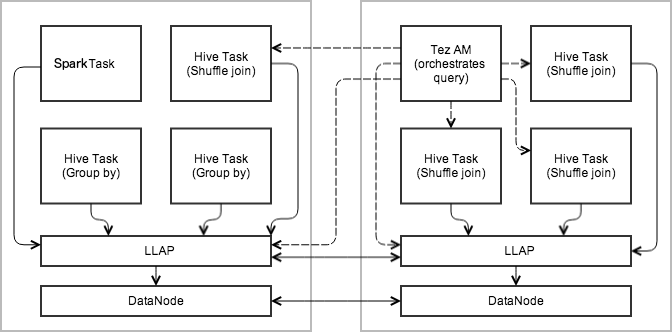
\includegraphics[width=\textwidth]{figures/arch1.png}
\caption{LLAP: as an accelerator}
\label{fig:arch1}
\end{figure*} 

The query engine remains Hive, running Hive
SQL operators while using Tez's DAG execution engine to execute the DAG across failure scenarios and to handle deadlock pre-emption within 
the DAG where multiple vertexes are in motion. This Hybrid execution model highlighted in Figure~\ref{fig:arch1}, in its simplest form 
converts LLAP into a tabular data reader service replacing direct interactions with the networked filesystem. While short running queries
can be run within LLAP entirely, the relational model offered by this interface into data is preferred over the file centric model which
can offer no security beyond file permissions. This change of roles allows for a process boundary between the user code executing within the 
hybrid tasks and allow LLAP to act as gatekeeper for columnar access control, column masking and cell level security.

\section{Cache}

\subsection{IO Elevator}

LLAP offloads I/O and transformation from compressed input to a set of threads referred to as the IO Elevator, as seen in Figure~\ref{fig:elevator}.
The IO elevator interacts with the networked storage in independent threads, which is triggered independently
of the operator pipeline initialization.  This operation starts reading from remote data stores into a cache 
buffer and works as a single split look-ahead pre-fetch, while the plan is initializing multi-vertex inputs
such as broadcast joins.
The 
IO elevator also evaluates any SARGs pushed down to the storage layer, effectively doing those operations 
out of the critical path for latency.
The IO elevator and the operator pipeline work through a small pool of vectorized row-batch buffers, organized
as a producer-consumer queue. The IO elevator places decoded batches into the pool, while the operator pipeline
consumes each batch and returns the batches to the elevator for disposal/reuse.

\begin{figure}[H]
\centering
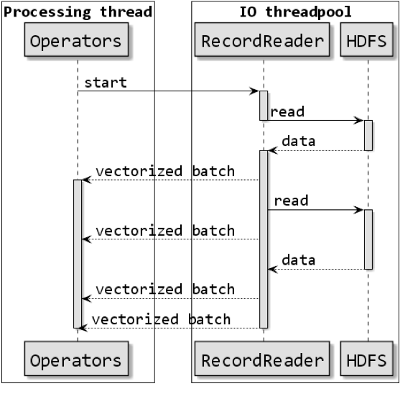
\includegraphics[width=0.8\columnwidth]{figures/elevator.png}
\caption{LLAP: IO Elevator}
\label{fig:elevator}
\end{figure} 

\subsection{Cache Addressing}

LLAP features an off-heap cache as its primary buffer pool for holding incoming data coming into
the IO elevator. The cache is addressed by the IO elevator along two dimensions, one along row-groups usually 10,000 rows and
the other along column order as showin in Figure~\ref{fig:cache_chunks}. The IO elevator reassembles the selected projection
and evaluates the predicates to extract column chunks which can be reconsitituted into the vector row-batches for the operator
pipeline. In case of cache misses, the cache is repopulated with the missing chunks before the reconsistution is performed,
simplifying the codepath and producing an incremental buildup of the cache as a user navigates the data-set along denormalized
dimensions, which is the common pattern the cache optimizes for.

\begin{figure}[H]
\centering
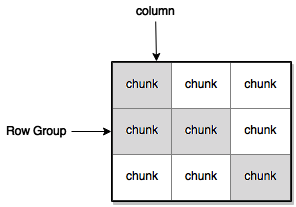
\includegraphics[width=0.8\columnwidth]{figures/cache-groups.png}
\caption{LLAP: Cache addressing}
\label{fig:cache_chunks}
\end{figure} 

LLAP cache holds within the metadata about input files as well as the data. The metadata and index information is cached even 
for data that was never in the cache. This is used to determine the row-groups that have to be loaded and to evaluate predicates
against the metadata before determining cache misses for the column chunks. With this in place, the first scan populates the indexes
in bulk and navigating within a dimension will not have to thrash the cache with column chunks which are effectively index misses.

To maintain validty of the cache, in the presence of updates, the cache lookup uses the HDFS FileId as the unique identifier to 
differentiate files of the same name which have different lineages. For extra strength, this combined with the length of the file
to detect appends to a file and for other fileystems, there are strong consistency equivalents to the FileId such as the ETag 
fields present in blob stores like Amazon S3\cite{S3} or Azure WASB\cite{WASB}. 

\subsection{Cache Policies \& Eviction}

The Cache eviction is also addressed at the same level as the addressing model, with each of those being evicted individually based
on the policy. The policy itself is pluggable, the initial policies available are LRFU and FIFO. The LRFU model is suitable for analytical
workloads with frequent partial table-scans, where retaining frequently used columns can provide cache hits if the projections in the
workload is popular.

\begin{figure}[H]
\centering
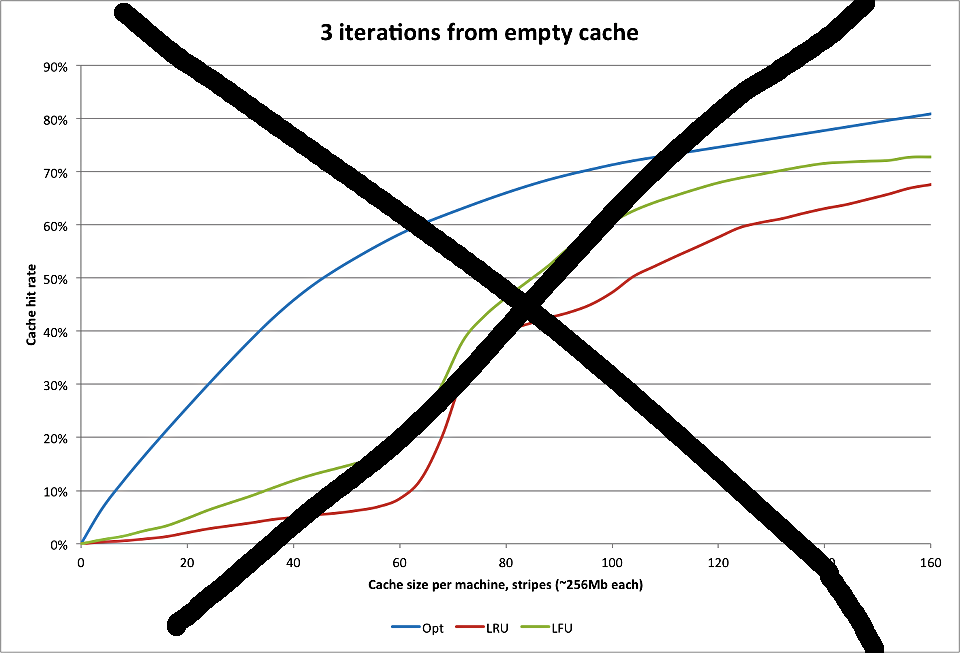
\includegraphics[width=0.8\columnwidth]{figures/evictions.png}
\caption{LLAP: Cache Policies}
\label{fig:eviction}
\end{figure} 

The cache internally uses a BuddyAllocator which handles the fragmentation issues that stem from evictions. The Allocator divies all
allocations into a series of Arenas, with each arena not being bigger than \emph{2Gb} in size due to 32 bit limitations in 
the off-heap APIs. Since the adjacent free blocks are always merged, the cache eviction does not return any memory to the system unlike
the buffer pools, therefore it will reuse the address space for future allocations. LLAP does not use the non-volatile nature of NVMe/NVMDIMM
backed caches, preferring to reinintialize the cache on restarts, which removes any potential wear-levelling concerns the BuddyAllocator
brings in by reusing blocks.

%% (TODO: discuss fallocate fl_hole_punch as a way of triggering TRIM for garbage).

\section{Deploy \& Elasticity}

LLAP is designed to run as a YARN application packaged by Apache Slider\cite{slider}, not as a daemon deployed by system installers. This brings multiple advantages within a Hadoop-2 cluster, first of which is that 
LLAP can be deployed and administered by a user who does not have access to any worker node on the cluster. The fact that YARN allocates containers and can possibly migrate away
from a blacklisted or decommisioning node provides automatic self-healing to the LLAP cluster, where a new container will take the place of one which has fallen without any user
intervention.

To cope in such a dynamically shifting environment, LLAP has had to build its own cluster membership protocols. The cluster membership is published through the YARN Service Registry or the 
alternate Zookeeper implementation keeps track of all existing LLAP nodes without a centralized master service to locate nodes. The service registry forms the discovery mechanism for the
orchestration systems which need to locate LLAP instances, obtain instance configuration from them and react to nodes being respawned elsewhere.

The dynamic discovery protocols and the existing failure tolerance models required to handle machine failures form the two pillars on which LLAP achieves elasticity based on user schedules. 
One of the common cost-efficiency problems for analyst driven BI tools is that they're wasted capacity, idling through out the non-office hours.  LLAP can \emph{flex} up and down within the
cluster to free up capacity during the off-hours for the cluster to be put to better use and for batch workloads.

This elasticity model has been designed so that this can happen without any user commands at all and can be purely controlled with a queue reservetion schedule within the YARN resource manager, as described in Microsoft Rayon paper \cite{rayon}.

\section{Query Fragments}

LLAP does not take up the responsibility of performing task orchestration or determining where each task should run on. 
This however is not possible directly by an external DAG engine such as Apache Tez\cite{tez}, without having access to
a common vocabulary for interaction. LLAP from the orchestration engine's perspective is another implementation of the
ContainerLauncher, but in this case one which talks to LLAP instance over rpc instead of the YARN NodeManager. Hive and
Tez together come up with a DAG plan, which is then divided into many query fragments which are self-contained and can 
execute on any LLAP instance, but has a definite preference towards cache affinity and HDFS data locality.

The fragments are scheduled onto LLAP daemons published under a name in the service registry. For the sake of enabling 
Hybrid execution mode, the events streaming out of LLAP are exactly identical to the events obtained from the Tez containers
and handled by a plugin service loaded into Tez ApplicationMaster. LLAP however receives some special events from the
plugin when communicating downstream, since there are special indicators for clean up operations for queries which have
completed.

The query fragments kick off the IO elevator and initialize the operator pipeline in parallel. In some cases, the fragments
might discover that other fragments which require similar initialization are running in the same process and decide to 
co-operate on expensive initialization operations like building broadcast-join hashtables, which will be built exactly once
per node instead of being build multiple times in each fragment. If a query fragment happens to be waiting on a machine the
fragment will send heartbeats out eventhough it is not running, to let the DAG master know that the process hosting the
fragment is still alive.

The query fragments are the basic unit of failure tolerance. Whenever a query fragment fails, it gets rescheduled until it
has failed for the maximum number of times, the process of rescheduling it can even involve terminating a running fragment
which is part of the same query depending on the priority between the fragments. These operations within a single DAG execution
maps exactly to the dead lock prevention already in the Tez vertex manager plugins, differing only in the means of communication -
however, the speed at which LLAP fragments execute result in far higher likelihood of exposing race conditions within future 
vertexmanager plugins.


In secure clusters, the orchestration \& discovery can only happen with a single user, to avoid accidental security leakage
between users inhabiting the same process and sharing the same cache. This is not as much hardship as it sounds as the 
Apache Ranger\cite{ranger} perimeter security translates all users into a single user after security verifications are 
complete, to ensure that no user has actual file level access to tables.

\section{Concurrency Control}

LLAP is designed for busy clusters. This translates into a deluge of query fragments hitting each LLAP instance 
usually exceeding the capacity available on that node. Since cache locality is rather important, even after 
capacity of a node is occupied, it will maintain wait list of tasks which would be used a queue to pick the 
next task from instead of performing a full round-trip to the application masters. After all the executors are
full and the wait list is entirely taken  up, LLAP will start to turn away application masters and effectively
communicate a back-off to any query which wants to add more fragments to this specific node.

To get better throughput rather than low latency of return, increasing the depth of the wait queue will 
produce a system which is better at absorbing query fragments and executing them as resources become available,
resulting in an entirely busy system at all time. Alternatively, for a low latency query pattern, switching the locality delay to infinity for the cache affinity
will result in a task being pinned a node which has a high probablity of cache hit-rate, even if none of the machines
involved in the LLAP cluster have data locality. 

The wait queue and the forced affinity are both tuning parameters, which have differing effects in a busy cluster but in an entirely
idle cluster, they're both ways of ensuring that tasks run on the preferred nodes which have a high probability of cached data.


The wait queue is not a simple queue or even a static priority queue, the wait queue contains query fragments which have multiple
states of readiness as well as priority hueristics which change depending on how long it has been in the queue and how many of its 
siblings are complete. 

%% TODO: describe isFinishable, priority shifts 

\section{Experiments \& Takeaways}

Before dissecting the internals of LLAP, we take a brief digression into deployments and experiments, 
which add colour to the architectural discussions. 

\subsection{Yahoo Display Network Benchmark}

Yahoo Japan published a timeseries reporting business case as part of a benchmark\cite{impala_perf} comparing
latencies of Cloudera Impala\cite{impala} against Apache Hive. This use-case was based on a production scenario
which features a 500 billion row warehouse which has significant skews in its data distribution. The challenge 
described in the use-case stemmed from having both throughput and latency SLAs and simulated concurrent users
creating extracted reports for further analysis.

The use-case divided produced aggregate of metrics bounded by segments, of selected attributes. The segments 
were primarily the start of the period and the length of the period - daily, weekly, monthly and yearly. The 
attributes were selection criteria which included user demographics and object identifiers. This does not 
easily map into a pre-aggregate MOLAP system as the total number of object identifiers were very large and 
the join against total dimensions produced very little reduction in data, when maintained on a daily basis for
a year.

The query pattern for the time-series had a skew towards the last day and last week, which affects a MPP share-nothing
model adversely by producing a CPU hot-spot around the machines holding the last billion rows. Eventhough Tez was not
affected by that specific issue due to locality delay scheduling, it was still producing secondary network hotspots
around the storage nodes which contained more popular user-demographics. 

This experiment gave valuable feedback into the design of LLAP. Along with use of Tez sessions, the benchmark 
reached an acceptable 5.67 queries per second (20412 queries per hour, exceeding the 15000 queries per hour SLA).

As part of validating LLAP's solution, the exact same benchmark was setup with the latest Hive and run through for the following
query patterns with 20 users, each user getting a unique tuple of parameters.

\begin{itemize}
\item \textbf{Query1x}: aggregate by object id
\item \textbf{Query2x}: aggregate by day
\item \textbf{Query6x}: across 50 object ids by device
\item \textbf{Query7x}: across 50 object ids by day
\end{itemize}

The experimental 50 node cluster had machines with 10Gigabit Ethernet, 20 cores, 128Gb of RAM and 12 disks in each. The LLAP instances
were configured to utilize 96Gb per node, running 24 threads in total with a 10Gb cache. For the purpose of the benchmark, all logging
in LLAP was turned to WARN level to reduce IO overheads. All queries were executed from a single gateway node, over JDBC connections 
and latencies measured are seconds for JDBC submission till last row.

\iffalse
\begin{table}[h]
\begin{tabular}{l|*{4}c}
Query1x  &   Tez (avg)  &   Tez (worst)  &   LLAP (avg)  &   LLAP (worst) \\
\hline
One Day  &   2.53  &   4.5  &   1.33  &   3 \\
One Week  &   3  &   6.18  &   1.37  &   2.9 \\
One Month  &   4  &   7.28  &   1.35  &   2.7 \\
One year  &   7.4  &   19.51  &   3  &   17.22 \\
\end{tabular}
\caption{Query1x across different periods (s)}
\end{table}

\begin{table}[h]
\begin{tabular}{l|*{4}c}
Query2x  &   Tez (avg)  &   Tez (worst)  &   LLAP (avg)  &   LLAP (worst) \\
\hline \\
One Day  &   2.556  &   6.67  &   1.11  &   1.74 \\
One Week  &   1.99  &   2.84  &   1.01  &   1.47 \\
One Month  &   3.07  &   6.65  &   1.29  &   2.2 \\
One year  &   5.03  &   7.47  &   1.74  &   4.67 \\
\end{tabular}
\caption{Query2x across different periods (s)}
\end{table}

\begin{table}[h]
\begin{tabular}{l|*{4}c}
Query6x  &   Tez (avg)  &   Tez (worst)  &   LLAP (avg)  &   LLAP (worst) \\
\hline \\
One Day  &   1.9  &   2.6  &   1.17  &   3.63 \\
One Week  &   2.22  &   5.9  &   1.03  &   1.66 \\
One Month  &   3.5  &   6.7  &   1.23  &   2.76 \\
One year  &   6  &   7.27  &   2  &   5.44 \\
\end{tabular}
\caption{Query6x across different periods (s)}
\end{table}

\begin{table}[h]
\begin{tabular}{l|*{4}c}
Query7x  &   Tez (avg)  &   Tez (worst)  &   LLAP (avg)  &   LLAP (worst) \\
\hline \\
One Day  &   1.9  &   2.6  &   1.17  &   3.63 \\
One Week  &   2.22  &   5.9  &   1.03  &   1.66 \\
One Month  &   3.5  &   6.7  &   1.23  &   2.76 \\
One year  &   6  &   7.27  &   2  &   5.44 \\
\end{tabular}
\caption{Query7x across different periods (s)}
\end{table}
\fi

\begin{figure}[bthp]
\centering
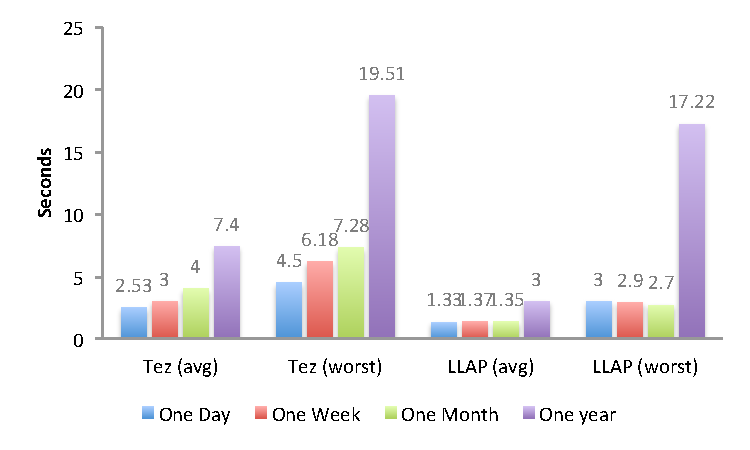
\includegraphics[width=0.9\columnwidth]{figures/q1x.pdf}
\caption{Query1x across different periods (s)}
\label{fig:q1x}
\end{figure} 

\begin{figure}[bthp]
\centering
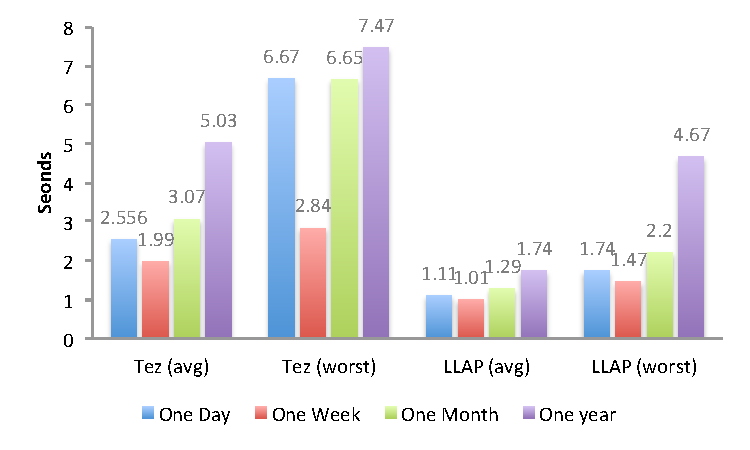
\includegraphics[width=0.9\columnwidth]{figures/q2x.pdf}
\caption{Query2x across different periods (s)}
\label{fig:q2x}
\end{figure} 

\begin{figure}[bthp]
\centering
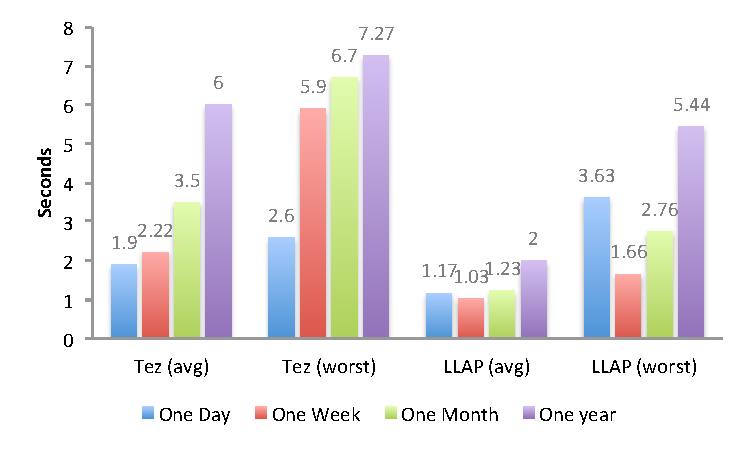
\includegraphics[width=0.9\columnwidth]{figures/q6x.pdf}
\caption{Query6x across different periods (s)}
\label{fig:q6x}
\end{figure} 

\begin{figure}[bthp]
\centering
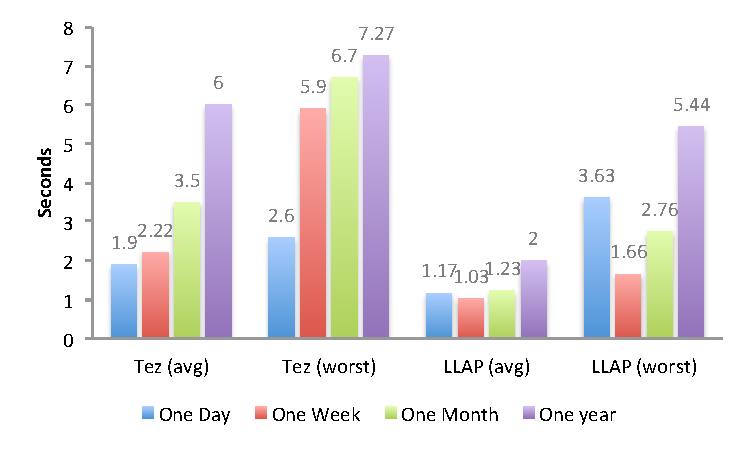
\includegraphics[width=0.9\columnwidth]{figures/q7x.pdf}
\caption{Query7x across different periods (s)}
\label{fig:q7x}
\end{figure} 


LLAP managed to lower the latency as well as hit a far higher throughput of 15.16 q/s (54576 queries per hour). The 
performance bottlenecks with LLAP had moved from the data skew towards the cpu utilized by the bottlenecks within
the JDBC layer in HiveServer2. This was isolated from the use-case by increasing the total number of users in the system and
increasing the number of HiveServer2 until worst case latencies dropped out of SLA.


\begin{figure}[!h]
\centering
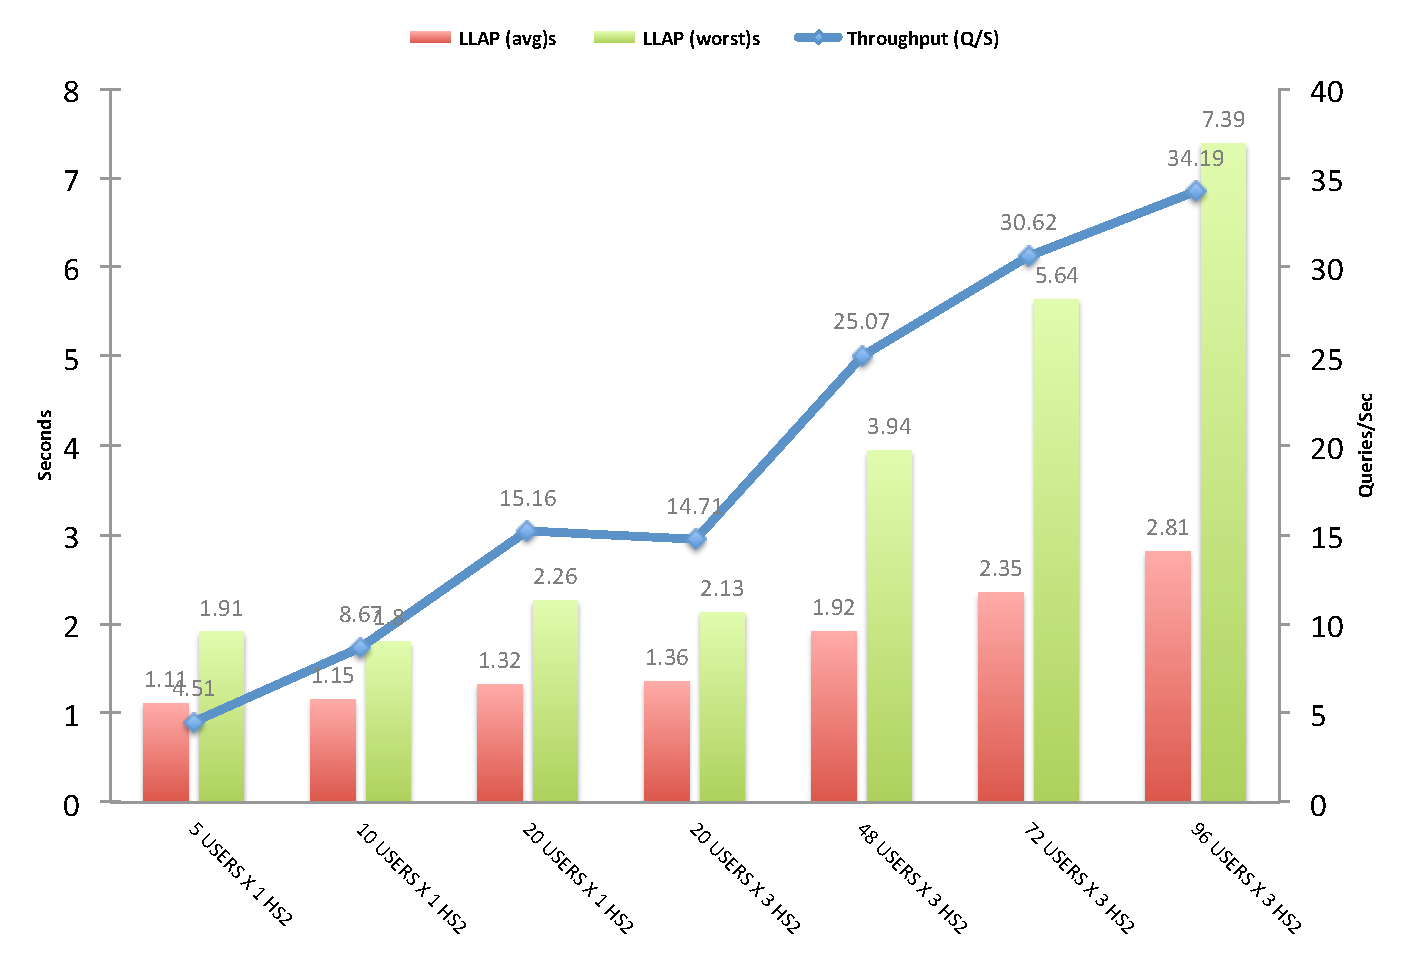
\includegraphics[width=0.9\columnwidth]{figures/throughput.pdf}
\label{fig:throughput}
\caption{HiveServer2 Concurrency Tests}
\end{figure}

\iffalse
\begin{table}[H]
\begin{tabular}{l|*{3}c}
Concurrency & Throughput (Q/S) & LLAP(avg)s & LLAP (worst)s \\
\hline \\
5 Users x 1 HS2 & 4.51 & 1.11 & 1.91 \\
10 Users x 1 HS2 & 8.67 & 1.15 & 1.8 \\
20 Users x 1 HS2 & 15.16 & 1.32 & 2.26 \\
20 Users x 3 HS2 & 14.71 & 1.36 & 2.13 \\
48 Users x 3 HS2 & 25.07 & 1.92 & 3.94 \\
72 Users x 3 HS2 & 30.62 & 2.35 & 5.64 \\
96 Users x 3 HS2 & 34.19 & 2.81 & 7.39 \\
\end{tabular}
\caption{HiveServer2 Concurrency Tests}
\end{table}
\fi

\subsection{TPC-DS Interactive Queries}

\begin{figure}[bthp]
\centering
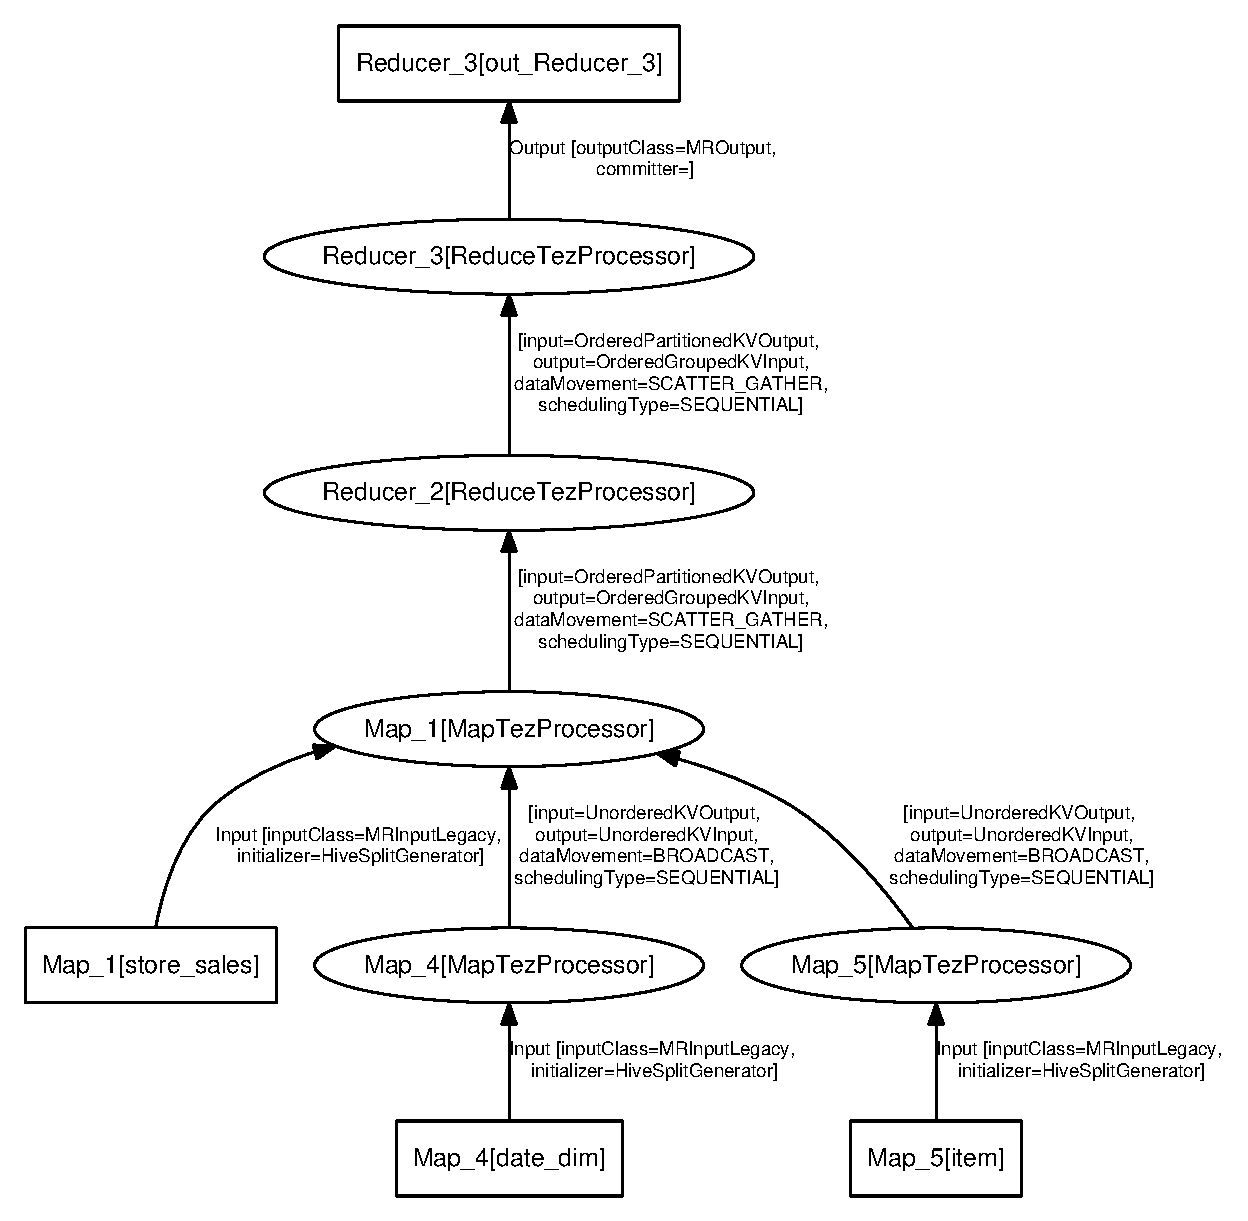
\includegraphics[width=0.8\columnwidth]{figures/q55.eps}
\caption{Query55: DAG Plan}
\label{fig:q55}
\end{figure} 

The TPC-DS data-set is a better candiate for a repeatable benchmark for LLAP, allowing any cluster to generate
identical data at scale factors for testing. The experimental setup is a \emph{SCALE=1000} TPC-DS data set generated
and loaded using the schema from hive-testbench\cite{testbench}, with interactive set of 27, 42, 52, 55, 68, 73 and 98, 
without introducing any partition filters on the queries.

These are all multi-stage queries from a MapReduce context, with internal shuffle distribution edges. For example, 
Query 55 DAG plan is illustrated in figure~\ref{fig:q55}.  

Benchmarked on a Hadoop 2.7.1 cluster, with following hardware configuration.

\begin{itemize}
\item 2x Intel(R) Xeon(R) CPU E5-2640 v2 @ 2.00GHz for total of 16 CPU cores/machine
\item 256GB RAM per node
\item 6x 4TB WDC WD4000FYYZ-0 drives per node
\item 10 Gigabit interconnect between the nodes
\end{itemize}

The LLAP instances were created with 128Gb of working set memory, 32Gb of cache and 16 executor threads per
instance. The following configurations were applied to the Hive planner to produce consistent cache coherent 
runs during benchmarking.

\begin{itemize}
\item hive.llap.task.scheduler.locality.delay=-1;
\item hive.llap.client.consistent.splits=true;
\item hive.optimize.reducededuplication.min.reducer=1;
\end{itemize}

\iffalse
\begin{table}[h]
\begin{tabular}{l|*{1}cr}
Query & LLAP time(s)\\
\hline \\
Query 27 & 3.13  \\
Query 42 & 0.98  \\
Query 52 & 1.05  \\
Query 55 & 1.76  \\
Query 68 & 4.77  \\
Query 73 & 1.90  \\
Query 98 & 5.36  \\
\end{tabular}
\caption{Interactive Queries on LLAP}
\end{table}
\fi

\begin{figure}[bthp]
\centering
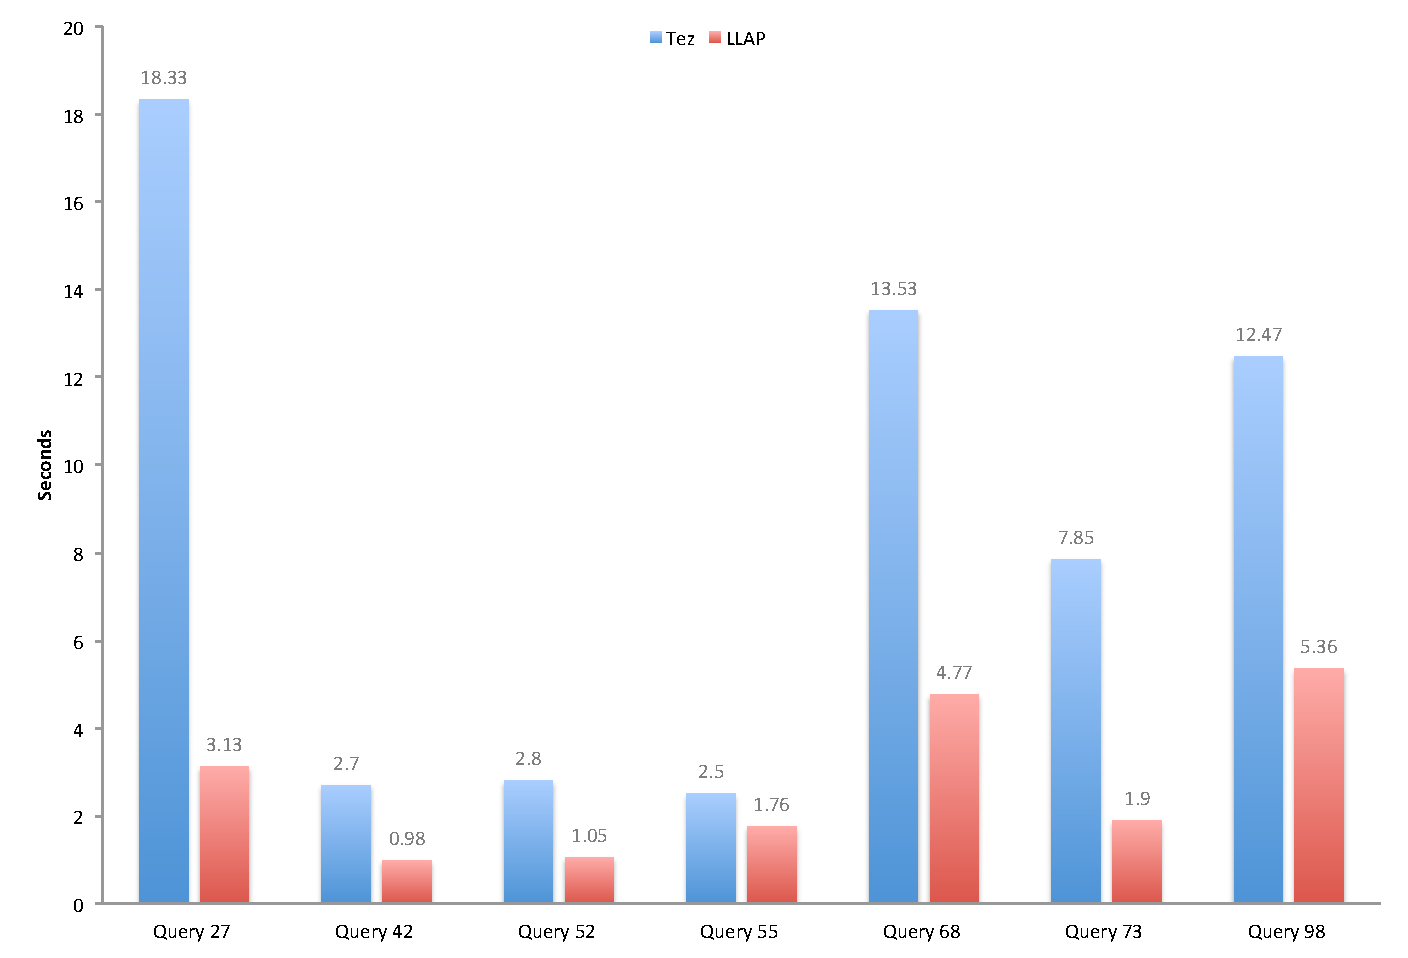
\includegraphics[width=0.8\columnwidth]{figures/tpc-ds.pdf}
\caption{Interactive queries: LLAP vs Tez}
\label{fig:llap_v_tez}
\end{figure} 

The queries 42, 52 \& 55, can run at the similar latencies even when using a single LLAP instance to compare against, since they process
approximately 93 million rows, which is less than the single node processing rate of LLAP clocked at approximately 115 million rows per second  
for ORC.

\section{Future Work}

\subsection{Spark integration}

Column masking, cell masking for SparkSQL

\subsection{ACID Transactions}

Support for streaming ingest caching.

\subsection{NVDIMM Cache Restart}

Preserve cache across restarts


\section{Related Work}

\subsection{HBase metastore}

Better statistics, orc splits cache, DPP in metastore

\subsection{CBO}

Faster planning 

\subsection{ODBC Driver Performance}

Should be able to read the first row faster via HiveServer2 JDBC.

\section{Conclusions}

LLAP is here along with hive-2.0, for anyone to try it out.



\section*{Acknowledgements}
Apache Hive is an open source community driven project with contributions gratefully accepted from numerous individuals and organizations. 
In particular we would like to call out ...
We are also grateful to Yahoo Japan, Microsoft Azure and Hortonworks for providing experimentation infrastructure. 

\balance
\small
\bibliographystyle{abbrv}
\bibliography{biblio}

\end{document}
